\documentclass{beamer}

\usepackage{amsmath}
\usepackage{amssymb}
\usepackage{graphicx}
\usepackage{subcaption}
%\usepackage{subfigure}
\usepackage{float}
\usepackage{multirow}
\usepackage{alphalph}
\usepackage{lipsum}


%\usepackage{geometry}[width=5in,height=3.75in]
%\usepackage{animate}
% \usepackage{multimedia}
%\usepackage{caption}



\usepackage{appendixnumberbeamer}
\usetheme{Frankfurt}
%\xdefinecolor{maroon}{cmyk}{0.15,1.00,0.39,0.69}
%\xdefinecolor{maroon}{cmyk}{0.27,0.86,0.60,0.30}
%\xdefinecolor{maroon}{cmyk}{0.000,1.00,1.00,0.498}
\usecolortheme[RGB={80,0,0}]{structure}

% Shortcut commands
% My Shortcut Commands
\newcommand{\fig}[1]{Fig.~\ref{#1}}                      % figure
\newcommand{\tbl}[1]{Table~\ref{#1}}                     % table

\newcommand{\be}{\begin{equation*}}   % numbered equation
\newcommand{\ee}{\end{equation*}}

\newcommand{\benum}{\begin{equation}}   % numbered equation
\newcommand{\eenum}{\end{equation}}

\newcommand{\bea}{\begin{eqnarray*}}  % numbered equation array
\newcommand{\eea}{\end{eqnarray*}}

\newcommand{\beanum}{\begin{eqnarray}}  % numbered equation array
\newcommand{\eeanum}{\end{eqnarray}}

\newcommand{\eqt}[1]{Eq. (\ref{#1})}  % Reference to one equation
\newcommand{\eqts}[1]{Eqs. (\ref{#1})}  % Reference to multiple equations 

\newcommand{\vect}[1]{\ensuremath{ \vec{\mathbf #1}}}  % bold faced with vector arrow above
\newcommand{\B}[1]{\ensuremath{B_{#1} }}			% B with a sub scripted argument

\newcommand{\p}{\ensuremath{ \partial}}			% shortcut partial derivative symbol

\newcommand{\abs}[1]{\ensuremath{\left\lvert #1 \right\rvert}}  % absolute value of argument (variable bar size)
\newcommand{\norm}[1]{\ensuremath{\left\lVert #1 \right\rVert}}  % norm of argument, varaible size

\newcommand{\omg}{\ensuremath{\vec{\Omega}}}
\newcommand{\BCSZ}{\ensuremath{\widetilde{\psi}_{BCSZ}}}
\newcommand{\BCSZH}{\ensuremath{\widehat{\psi}_{BCSZ}}}

% Equation Punctuation
\newcommand{\pec}{\, ,}
\newcommand{\pep}{\, .}
\setbeamertemplate{footline}{
\leavevmode%
\hbox{\hspace*{-0.06cm}
\begin{beamercolorbox}[wd=.45\paperwidth,ht=2.25ex,dp=1ex,center]{author in head/foot}%
	\usebeamerfont{author in head/foot}Maginot Ragusa Morel (TAMU)%~~(\insertshortinstitute)
\end{beamercolorbox}%
\begin{beamercolorbox}[wd=.3\paperwidth,ht=2.25ex,dp=1ex,center]{section in head/foot}%
M\&C 2015 %\usebeamerfont{section in head/foot}\insertshorttitle
\end{beamercolorbox}%
\begin{beamercolorbox}[wd=.25\paperwidth,ht=2.25ex,dp=1ex,right]{section in head/foot}%
	\usebeamerfont{section in head/foot}April 20, 2015\hspace*{2em}
	\insertframenumber{} / \inserttotalframenumber\hspace*{2ex}
\end{beamercolorbox}}%
\vskip0pt%
}
\beamertemplatenavigationsymbolsempty
\beamertemplatetransparentcovered

\setbeamertemplate{bibliography item}[text]

\title{A Non-Negative Bilinear DFEM Scheme for $S_N$ Transport}
\author{Peter Maginot \\ Jean Ragusa and Jim Morel}\institute{Texas A\&M University- Department of Nuclear Engineering}
\date{M\&C 2015 \\ April 20, 2015 }


\newif\ifplacelogo % create a new conditional
\placelogotrue % set it to true
\logo{\ifplacelogo
\includegraphics[height=1cm]{CSGF_vert.pdf} \hspace{3.5in} 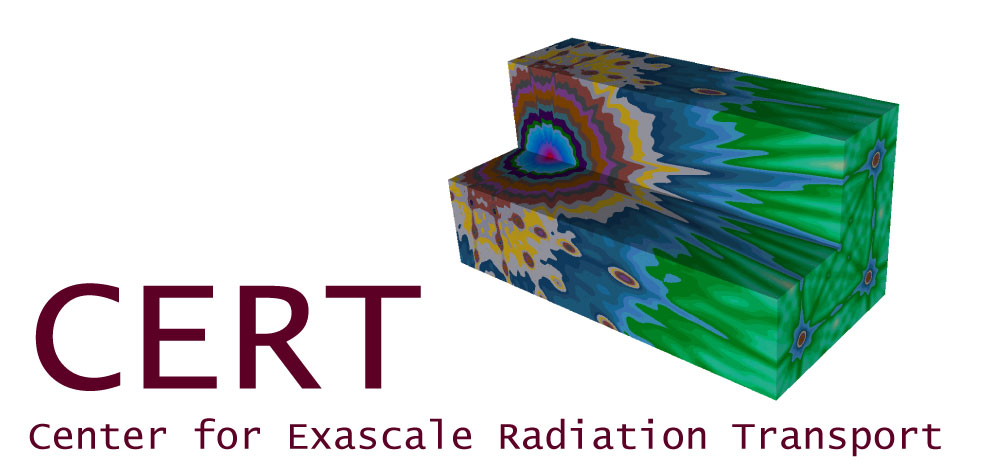
\includegraphics[height=1cm]{cert-logo}\fi}

\begin{document}
%---------------------------------------------------------------------------------------------
\placelogotrue
\begin{frame}
\titlepage


\end{frame}

%---------------------------------------------------------------------------------------------

\placelogofalse
%---------------------------------------------------------------------------------------------

\begin{frame}
\frametitle{Outline}

\begin{enumerate}
\item Goal/Motivation
\item Basics
\item BCSZ Method
\item Initial Results
\end{enumerate}

\end{frame}

%---------------------------------------------------------------------------------------------

\section{Goal}

\subsection{Goal}
\begin{frame}
\frametitle{Goal}
Long term goal: Accurate methods for multi-dimensional radiative transfer
Near term goal: Non-negative bilinear DFEM for neutron transport
-Why bilinear? Bilinear DFEM maintains thick diffusion limit, radiative transfer requires optically thick cells
History: Extension of non-negative linear $(1,x,y)$ scheme developed on rectangles
\end{frame}

%---------------------------------------------------------------------------------------------

\section{Basics}

\subsection{DFEM Basics}

\begin{frame}
\frametitle{Formalities}
Solving
\benum
\omg_d \cdot \nabla \psi_d(x,y) + \sigma_t(x,y) \psi_d(x,y) = S_d(x,y)
\label{eq:transport}
\eenum
for unstructured quadrilaterals using bilinear ($Q^1$) DFEM.

\begin{itemize}
\item Using the standard interpolatory basis functions
\end{itemize}
\bea
\B{0}(s,t) &=& \frac{1-s}{2}\frac{1-t}{2} \\
\B{1}(s,t) &=& \frac{s+1}{2}\frac{1-t}{2} \\
\B{2}(s,t) &=& \frac{s+1}{2}\frac{t+1}{2} \\
\B{3}(s,t) &=& \frac{1-s}{2}\frac{t+1}{2}  
\eea

\end{frame}

%---------------------------------------------------------------------------------------------

\subsection{Geometry Mapping}
\begin{frame}
\frametitle{Mapping to Reference Coordinates}
All work carried out on a reference element, $s\in[-1,1]~,t\in[-1,1]$
\begin{figure}[t]
\centering
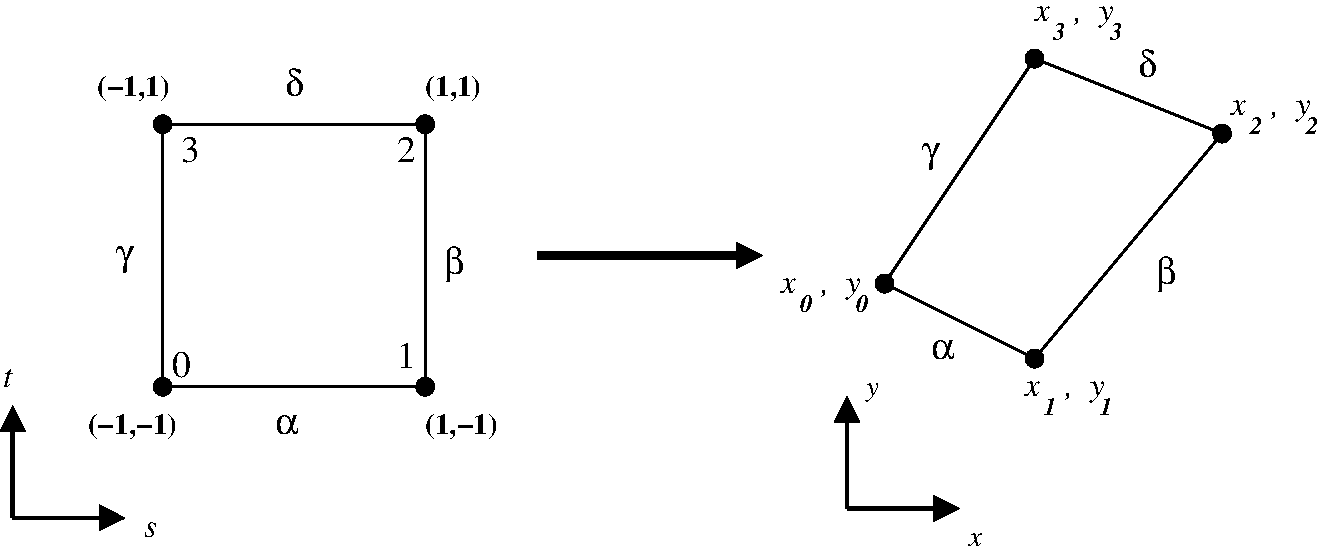
\includegraphics[width=3in]{mc_coord.pdf}
\end{figure}
%
%
\beanum
x &=& x_0 \B{0}(s,t) + x_1 \B{1}(s,t) + x_2 \B{2}(s,t) + x_3 \B{3}(s,t) \\
y &=&  y_0 \B{0}(s,t) + y_1 \B{1}(s,t) + y_2 \B{2}(s,t) + y_3 \B{3}(s,t) 
\eeanum
\end{frame}

\begin{frame}
\frametitle{Methods to Compare}
\begin{enumerate}
\item UBLD: Unlumped Bilinear DFEM- Galerkin DFEM, no explanation necessary \vspace{0.2in}
\item FLBLD: Fully Lumped Bilinear DFEM- UBLD with mass matrix lumping, surface matrix lumping, and other manipulations.  Equivalent to sub-cell corner balance. \vspace{0.2in}
\item BCSZ: Bilinear consistent set-to-zero: Non-linear, Petrov-Galerkin DFEM, satisfies all bilinear moments of \eqt{eq:transport} 
\end{enumerate}

\end{frame}

%---------------------------------------------------------------------------------------------


\section{BCSZ Method}
\subsection{Definition}

\begin{frame}
\frametitle{BCSZ Definition}
Solution representation, $\widetilde{\psi}_{BCSZ}(s,t)$:
\benum
\BCSZ(s,t) = \left \{ \begin{array}{ll}
\BCSZH(s,t) & \BCSZH(s,t) > 0 \\
0	& \text{otherwise}
\end{array}
\right. \pep
\label{eq:bcsz}
\eenum
Bilinear function, $\widehat{\psi}_{BCSZ}$, to search for,
\benum
\BCSZH(s,t) = \sum_{i=0}^3{\psi_{i,BCSZ} \B{i}(s,t)} \pec
\eenum

\end{frame}

\subsection{Edge Integration}
\begin{frame}
\frametitle{Moment Equation Edge Integration}
DFEM moment equations will need to integrate quantities like this on cell edges:
\be
(\omg_d \cdot \vec{n}_{\alpha}) \int_{\alpha}{\B{i}(s,-1) \BCSZ~ds}
\ee
\begin{enumerate}
\item Check vertices for negativity
\item By definition of \BCSZ, integrate \BCSZH ~only over portion of the interval where $\BCSZH\geq 0$
\begin{itemize}
\item 4 possible cases
\end{itemize}
\end{enumerate}

\end{frame}

%---------------------------------------------------------------------------------------------

\subsection{Cell Integration}
\begin{frame}
\frametitle{Cell Interior Integration}
Must integrate terms like, $\B{i} \BCSZ \abs{J}$, over areas like these:
\begin{figure}[!hbp]
	\centering
	\begin{subfigure}{0.32\textwidth}
		\centering
		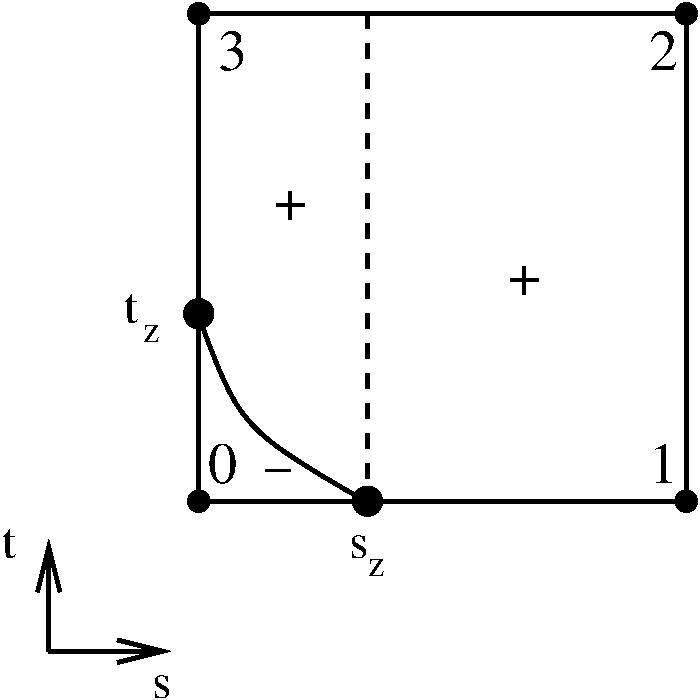
\includegraphics[width=1.2in]{one_neg_pdt_int} 		
  \end{subfigure}
	\begin{subfigure}{0.32\textwidth}
		\centering
		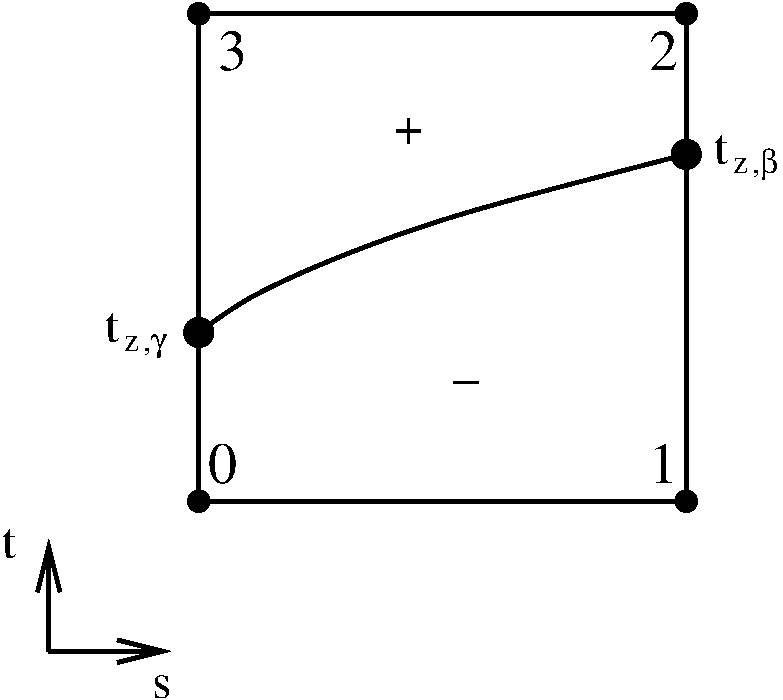
\includegraphics[width=1.2in]{neg_same_side_pdt_int}		
	\end{subfigure}
	\begin{subfigure}{0.32\textwidth}
		\centering
		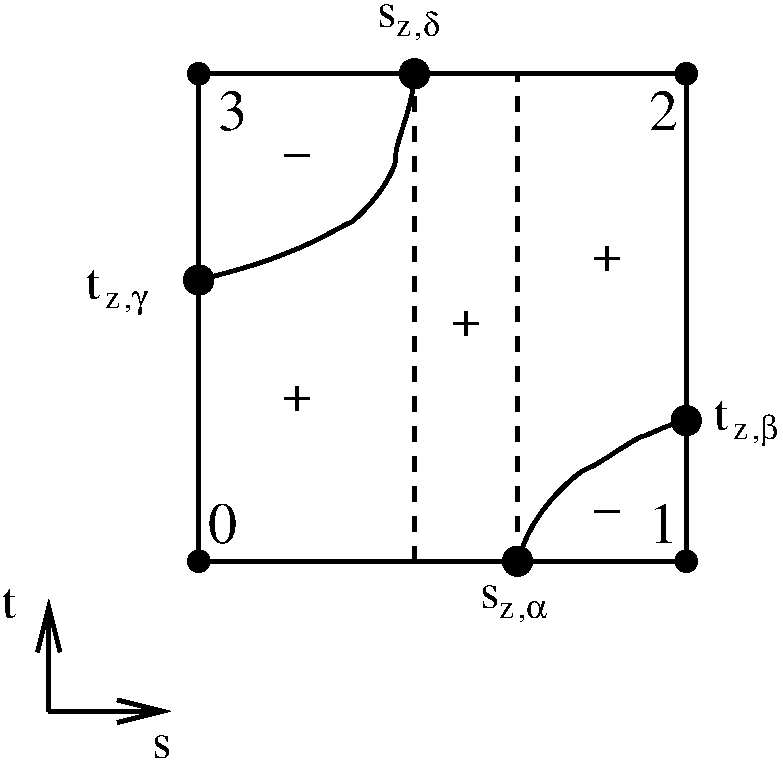
\includegraphics[width=1.2in]{opp_neg_more_pos_pdt_int}
	\end{subfigure}
	\begin{subfigure}{0.32\textwidth}
	\centering
		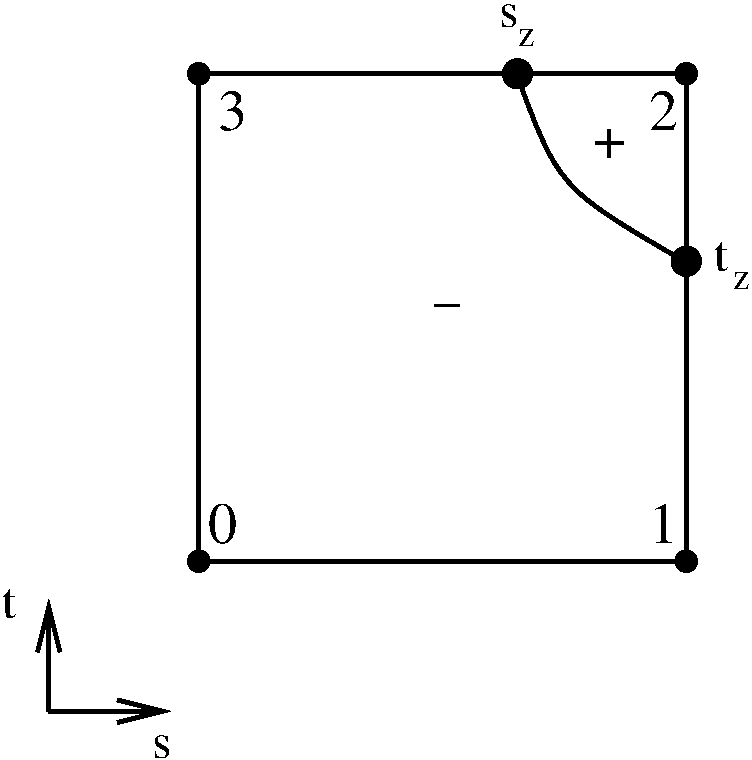
\includegraphics[width=1.2in]{three_neg_pdt_int} 
	\end{subfigure}
	\begin{subfigure}{0.32\textwidth}
		\centering
		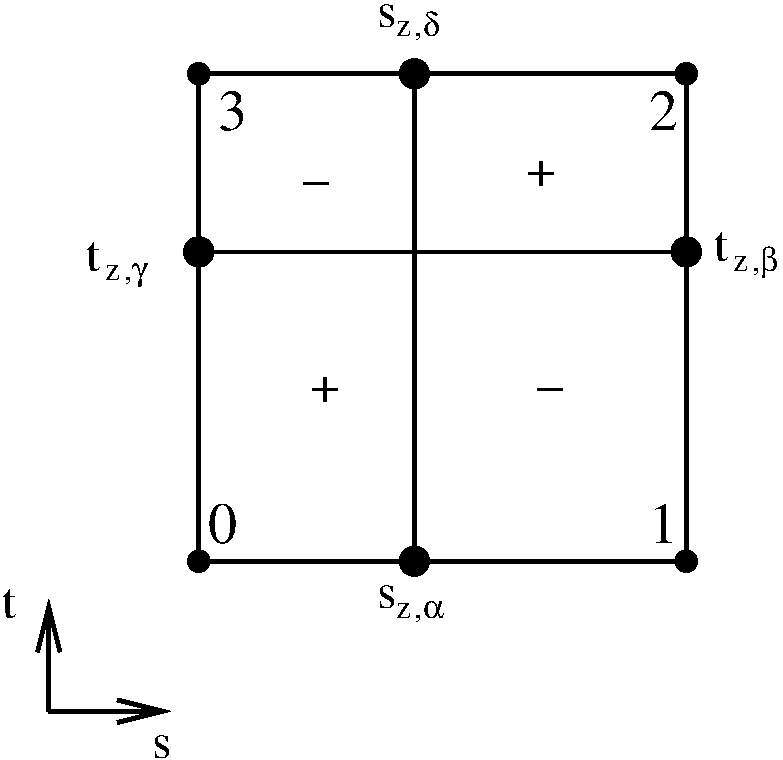
\includegraphics[width=1.2in]{opp_neg_block_pdt_int} 
	\end{subfigure}
	\begin{subfigure}{0.32\textwidth}
	\centering
		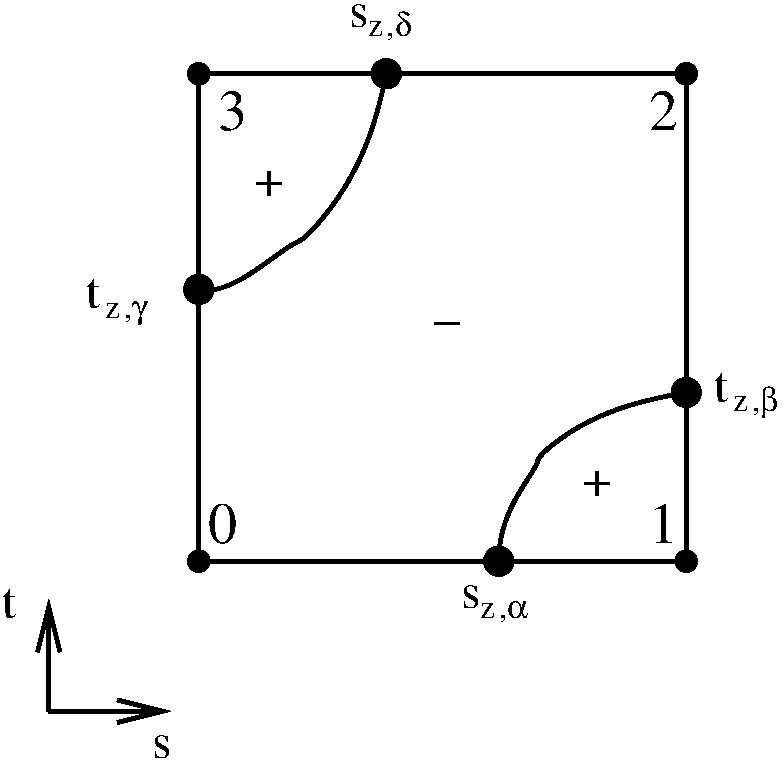
\includegraphics[width=1.2in]{opp_neg_more_neg_pdt_int}
	\end{subfigure}
\end{figure}

\end{frame}

\begin{frame}
\frametitle{Enabling Idea}
Along every integration area curve:
\be
\BCSZH(s,t) = 0
\ee
Transform interpolatory \BCSZH~ to moment based $f(s,t)$:
\benum
f(s,t) = f_c + s f_s + t f_t + st f_{st} 
\label{eq:f_def}
\eenum
\benum
\left[ 
\begin{array}{cccc}
1 &	 -1	& -1 &  1    \\
1 &		1	& -1	&  -1		\\	
1 &	  1	&  1		&  1		\\
1 &		-1	& 1		&  -1		\\
\end{array}
\right]
\left[
\begin{array}{c}
f_c \\
f_s \\
f_t \\
f_{st} 
\end{array}
\right]
=\vec{\psi}_{BCSZ}
\eenum

\end{frame}
%%%%%%%%%%%%%%%%%%%%%%%%%%%%%%%%%%
\begin{frame}
\frametitle{Enabling Idea- 2}

Along each integration area defined by a curve, $f(s,t) = 0$, and 
\benum
\hat{l}_t  = -\frac{f_c + f_s s}{f_t + f_{st} s} \pec
\eenum
enabling the use of variable limits of integration. 
Consider integration over the region where $\BCSZH>0$, $R_+$, of a generic function $M(s,t)$:
\begin{columns}[c]
\column{0.3\textwidth}
\begin{figure}
\centering
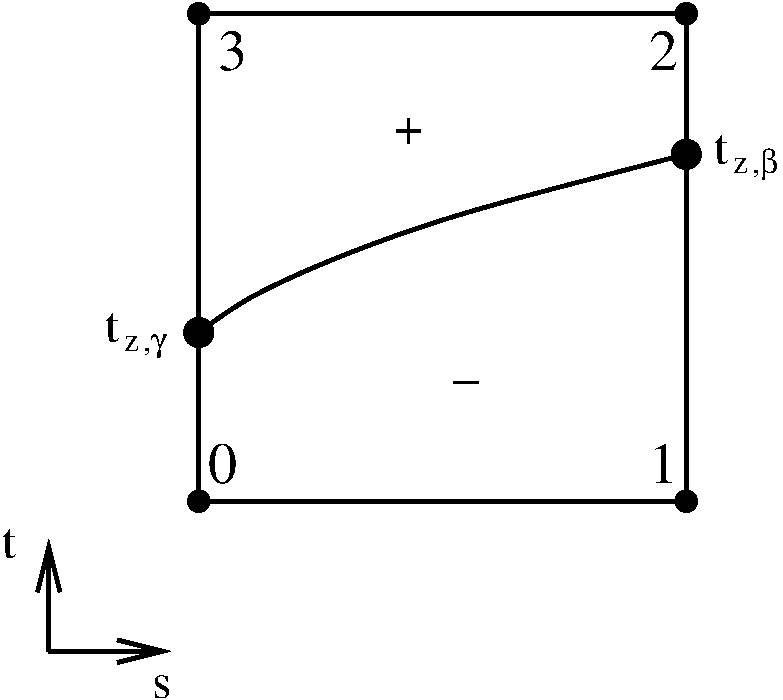
\includegraphics[width=1.25in]{neg_same_side_pdt_int} 
\end{figure}
\column{0.6\textwidth}
\be
\int{\int_{R_+}{ M(s,t) } } = 
\int_{-1}^{1}{ds~\int_{\hat{l}_t}^1{dt~M(s,t)} } 
\ee
\end{columns}
\end{frame}

\subsection{Almost Analytic Integration}

\subsection{Non-linear Iteration}

%---------------------------------------------------------------------------------------------

\section{Initial Computational Results}

%%%%%%%%%%%%%%%%%%%%%%%%%%%%%%%%%%%%%%%%%%%%%%%%%%%%%%%%%%%%%%%%%%%%%%%%%%%%%%%%%

\end{document}
%------------------------------------------------------------------------------